% !TeX encoding = UTF-8
% !TeX program = xelatex
% !TeX spellcheck = en_US

\documentclass[degree=master]{thuthesis}
  % 学位 degree:
  %   doctor | master | bachelor | postdoc
  % 学位类型 degree-type:
  %   academic(默认)| professional
  % 语言 language
  %   chinese(默认)| english
  % 字体库 fontset
  %   windows | mac | fandol | ubuntu
  % 建议终版使用 Windows 平台的字体编译


% 论文基本配置,加载宏包等全局配置
%\input{thusetup}


\begin{document}

% 封面
%\maketitle

% 学位论文指导小组、公开评阅人和答辩委员会名单
% 本科生不需要
%\input{data/committee}

% 使用授权的说明
% 本科生开题报告不需要
%\copyrightpage
% 将签字扫描后授权文件 scan-copyright.pdf 替换原始页面
% \copyrightpage[file=scan-copyright.pdf]

\frontmatter
% !TeX root = ../thuthesis-example.tex

% 中英文摘要和关键字

\begin{abstract}
  本文深入探讨了区块链技术的定义、原理、特点及其在现代社会中的重要意义。首先介绍了区块链的基本概念和核心技术构成,例如区块链的定义和优势,随后分析了区块链对数据安全、商业信任机制以及社会经济体系的潜在影响。并且进一步剖析了区块链的常见算法、面临的技术挑战、监管问题以及市场认知等关键问题。最后,通过分析区块链在不同领域的应用实践,展望了区块链技术的未来发展趋势,并讨论了不同国家区块链发展现状及其对社会环境的影响,以及重申了区块链的平行安全概念框架[社会物理信息系统 (Cyber-physical-social systems, CPSS)] [6].
  % 关键词用“英文逗号”分隔,输出时会自动处理为正确的分隔符
  \thusetup{
    keywords = {区块链, 数据安全, 技术分析, 发展历程, 监管},
  }
\end{abstract}

\begin{abstract*}
  This paper explores the definition, principles, characteristics and significance of blockchain technology in modern society. It first introduces the basic concepts and core technology components of blockchain, such as the definition and advantages of blockchain, and then analyzes the potential impact of blockchain on data security, business trust mechanisms and social and economic systems. It also further analyzes key issues such as common blockchain algorithms, technical challenges, regulatory issues and market perception. Finally, by analyzing the application practices of blockchain in different fields, it looks forward to the future development trend of blockchain technology, discusses the current status of blockchain development in different countries and its impact on the social environment, and reiterates the parallel security conceptual framework of blockchain [Cyber-physical-social systems (CPSS)] [6].
  \thusetup{
    keywords* = {Blockchain, Data Security, Technical Analysis, Development History, supervision},
  }
\end{abstract*}


% 目录
\tableofcontents

% 插图和附表清单
% 本科生的插图索引和表格索引需要移至正文之后、参考文献前
% \listoffiguresandtables  % 插图和附表清单(仅限研究生)
%\listoffigures           % 插图清单
%\listoftables            % 附表清单

% 符号对照表
%\input{data/denotation}


% 正文部分
\mainmatter
% !TeX root = ../thuthesis-example.tex

\chapter{了解区块链}

本章开头用简短的篇幅介绍了区块链的来源,
以及理解接下来的章节关于区块链的一些必要知识。

\section{区块链的定义与原理}

区块链是一种基于对等网络(P2P网络)和现代密码学的安全可信的公共分布式数据库,具有公开透明、去中心化、匿名性以及不可篡改等特点。

区块链以块的形式存储数据,并使用密码学方法保证数据的安全性和完整性。每个块包含一定数量的交易信息,并通过加密链接到前一个块,形成一个不断增长的链条。这种设计使得数据在网络中无法被篡改,因为任何尝试修改一个块的数据都会破坏整个链的连续性。通过去中心化的网络结构,区块链技术实现了对数据的分布式共享和管理,从而在不需要信任中介的情况下确保了数据的安全和可靠性。



\section{区块链的特点}

\subsection{去中心化}
	
去中心化:在中本聪的设计中,每一枚比特币的产生都独立于权威中心机构,任意个人、组织都可以参与到每次挖矿、交易、验证中,成为庞大的比特币网络中的一部分。区块链网络通常由数量众多的节点组成,根据需求不同会由一部分节点或者全部节点承担账本数据维护工作,少量节点的离线或者功能丧失并不会影响整体系统的运行。在区块链中,各个节点和矿工遵守一套基于密码算法的记账交易规则,通过分布式存储和算力,共同维护全网的数据,避免了传统中心化机构对数据进行管理带来的高成本、易欺诈、缺乏透明、滥用权限等问题。普通用户之间的交易也不需要第三方机构介入,直接点对点进行交易互动即可 [1]。

\subsection{开放性}
开放性:区块链系统是开放的,它的数据对所有人公开,任何人都可以通过公开的接口查询区块链数据和开发相关应用,因此整个系统的信息高度透明。虽然区块链的匿名性使交易各方的私有信息被加密,但这不影响区块链的开放性,加密只是对开放信息的一种保护 。

在开放性的区块链系统中,为了保护一些隐私信息,一些区块链系统使用了隐私保护技术,使得人们虽然可以查看所有信息,但不能查看一些隐私信息[1] 。

\subsection{开放性}
匿名性:在区块链中,数据交换的双方可以是匿名的,系统中的各个节点无须知道彼此的身份和个人信息即可进行数据交换 。
	
我们谈论的隐私通常是指广义的隐私:别人不知道你是谁,也不知道你在做什么。事实上,隐私包含两个概念:狭义的隐私(Privacy)与匿名(Anonymity)。狭义的隐私就是别人知道你是谁,但不知道你在做什么;匿名则是别人知道你在做什么,但不知道你是谁。虽然区块链上的交易使用化名(Pseudonym),即地址(Address),但由于所有交易和状态都是明文,因此任何人都可以对所有化名进行分析并建构出用户特征(User Profile)。更有研究指出,有些方法可以解析出化名与IP的映射关系,一旦IP与化名产生关联,则用户的每个行为都如同裸露在阳光下一般。

在比特币和以太坊等密码学货币的系统中,交易并不基于现实身份,而是基于密码学产生的钱包地址。但它们并不是匿名系统,很多文章和书籍里面提到的数字货币的匿名性,准确来说其实是化名。在一般的系统中,我们并不明确区分化名与匿名。但专门讨论隐私问题时,会区分化名与匿名。因为化名产生的信息在区块链系统中是可以查询的,尤其是在公有链中,可以公开查询所有的交易的特性会让化名在大数据的分析下完全不具备匿名性。但真正的匿名性,如达世币、门罗币、Zcash等隐私货币使用的隐私技术才真正具有匿名性。

匿名和化名是不同的。在计算机科学中,匿名是指具备无关联性(Unlinkability)的化名。所谓无关联性,就是指网络中其他人无法将用户与系统之间的任意两次交互(发送交易、查询等)进行关联。在比特币或以太坊中,由于用户反复使用公钥哈希值作为交易标识,交易之间显然能建立关联。因此比特币或以太坊并不具备匿名性。这些不具备匿名性的数据会造成商业信息的泄露,影响区块链技术的普及使用[1] 。
	
\subsection{可追溯性}
可追溯性:区块链采用带时间戳的块链式存储结构,有利于追溯交易从源头状态到最近状态的整个过程。时间戳作为区块数据存在的证明,有助于将区块链应用于公证、知识产权注册等时间敏感领域 [1]。

\subsection{透明性}
透明性:相较于用户匿名性,比特币和区块链系统的交易和历史都是透明的。由于在区块链中,账本是分发到整个网络所有参与者,账本的校对、历史信息等对于账本的持有者而言,都是透明的、公开的[1] 。

\subsection{不可篡改性}
不可篡改性:比特币的每次交易都会记录在区块链上,不同于由中心机构主宰的交易模式,其中心机构可以自行修改任意用户的交易信息,比特币很难篡改[1] 。

\subsection{多方共识}
多方共识:区块链作为一个多方参与维护的分布式账本系统,参与方需要约定数据校验、写入和冲突解决的规则,这被称为共识算法。比特币和以太坊作为公有链当前采用的是工作量证明算法(PoW),应用于联盟链领域的共识算法则更加灵活多样,贴近业务需求本身[1]。 









% !TeX root = ../thuthesis-example.tex

\chapter{区块链的意义}

\section{对数据安全与隐私保护的意义}

数据安全与隐私保护的现状堪忧:

1、(隐私数据方面)2024年上半年全网监测并分析验证有效的数据泄露事件16011起,较2023年下半年增长59.58%,共9539起[2];
2、(隐私数据方面)2024年上半年监测到3.4万个黑产团伙中,经分析验证涉及真实数据泄露事件的黑产团伙共计1973个,较2023年下半年增新增984个,增长近一倍[2];
3、(交易方面)从行业分布来看,2024年上半年数据泄露事件涉及85个行业,数据泄露事件数量Top5行业分别为银行、电商、消费金融、保险、快递[2]。;
4、(隐私数据方面)针对黑产数据交易市场研究发现,2024年上半年利用Facetime诈骗活动增多,2024年上半年泄露的数据中包含“IOS”字段的相关风险事件高达1237起,较2023年下半年增加8倍[2]。

隐私数据方面:区块链技术通过去中心化的特点增强了数据安全性,传统的数据存储通常集中在中心化的服务器上,这使得数据容易受到黑客攻击和数据篡改。而区块链技术将数据分布在网络的各个节点上,每一块数据都是通过加密算法链接在一起形成链式结构。这种去中心化的特点使得黑客很难入侵所有节点并篡改数据,因此增加了数据的安全性。

交易方面:区块链技术采用了强大的加密算法,保证了数据传输和存储的安全性每一笔交易都经过加密,只有特定的私钥持有者才能解密并访问数据。这使得数据在传输和存储中受到了强大的保护,即使数据被截获或泄露,黑客也无法获得有用的信息。同时,区块链上的数据只能被授权的用户修改和访问,其他人无法篡改或删除数据,确保了数据的完整性。

数据的匿名和隐私保护方面:传统的数据库存储个人信息或敏感数据时,通常需要用户提供真实姓名、身份证号码等个人身份信息。而区块链上的智能合约通过匿名特性,使得用户可以在不暴露真实身份的情况下进行交易和数据分享。智能合约使用密钥对验证身份,而无需暴露个人身份信息,确保了用户的隐私和数据的安全。

数据共享和溯源方面:传统的数据共享存在隐私泄露和数据篡改的问题,而区块链技术通过确保数据的真实性、不可篡改性和可追溯性,建立了可信任的数据共享机制。利用区块链技术,用户的个人数据可以得到充分保护的同时,还能够与其他用户安全地分享数据,促进信息的共享和交流。


%\begin{figure}
%  \centering
%  \includegraphics[width=0.5\linewidth]{example-image-a.pdf}
%  \caption*{国外的期刊习惯将图表的标题和说明文字写成一段,需要改写为标题只含图表的名称,其他说明文字以注释方式写在图表下方,或者写在正文中。}
%  \caption{示例图片标题}
%  \label{fig:example}
%\end{figure}

\section{对商业信任机制的影响}

在经济学的语境里,信任是一种行为策略,而信用可以被看做一个主观概率水平。只要潜在收益与守信行为的概率的乘积大于潜在损失与不守信的概率的乘积,信用就是占优势的行为策略。这是一个简单的信用表达式,但是可操作性很低。人并不是绝对理性的,而且不同的社会环境和制度会影响主体的选择。因此,难度最高的是构造出可以精确计算出行为的可信程度的系统。

但区块链的优越性正在于,通过精巧的设计,在这个系统内部,违约成本和预期收益可以被精确计算,因此理性个体将在权衡利弊后丧失欺诈的动力,从而一定程度优化商业信任机制。

\section{对社会和经济体系的潜在变革}

\subsection{对社会的潜在变革}

便捷司法存证,促进社会正义:

难点:在司法中,与传统司法证据相比,电子证据等的获取具有以下难点。
1.取证成本高。当前司法取证依赖于具有司法机制的存证机构,具有取证周期长、费用高等特点。同时人力投入大,操作成本较高。
2.取证难校验,公信力可能不足。由于电子证据本身易篡改、难溯源的特点,电子取证的权威性依赖于取证机构的资质与公信力,且取证后难以校验、追责。
2018年,我国公布了《最高人民法院关于互联网法院审理案件若干问题的规定》(以下简称《规定》)。《规定》第11条中明确规定:当事人提交的电子数据,通过电子签名、可信时间戳、哈希值校验、区块链等证据收集、固定和防篡改的技术手段或者通过电子取证存证平台认证,能够证明其真实性的,互联网法院应当确认。因此,区块链记录的电子证据可被认为是具有司法效力的证据,已有多个平台成功应用。

智能合同展新篇,社会合作换新颜:

区块链带来的智能合同实际上是在另一个物体的行动上发挥功能的计算机程序。与普通计算机程序一样,智能合同也是一种“如果—然后”的功能,但区块链技术实现了这些“合同”的自动填写和执行,无须人工介入。这种合同最终可能会取代法律行业的核心业务,即在商业和民事领域起草和管理合同的业务。

信息牢固于链连,政府透明社会安:

政务信息、项目招标等信息公开透明,政府工作通常受公众关注和监督,由于区块链技术能够保证信息的透明性和不可更改性,对政府透明化管理的落实有很大的作用。政府项目招标存在一定的信息不透明性,而企业在密封投标过程中也存在信息泄露的风险。区块链能够保证投标信息无法篡改,并能保证信息的透明性,在彼此不信任的竞争者之间形成信任共识。并能够通过区块链安排后续的智能合约,保证项目的建设进度,一定程度上防止了腐败的滋生。

\subsection{对经济体系的潜在变革}

供应链连商与户,经济监管减难度:

基于区块链的供应链金融应用中,通过将供应链上的每一笔交易和应收账款单据上链,同时引入第三方可信机构,例如银行、物流公司等,来确认这些信息,确保交易和单据的真实性,实现了物流、信息流、资金流的真实上链;同时,支持应收账款的转让、融资、清算等,让核心企业的信用可以传递到供应链的上下游企业,减小中小企业的融资难度,同时解决了机构的监管问题。

通过区块链进行数字资产交易,首先将链下资产登记上链,转换为区块链上的标准化数字资产,不仅能对交易进行存证,还能做到交易即结算,提高交易效率,降低机构间通信协作成本。监管机构加人联盟链中,可实时监控区块链上的数字资产交易,提升监管效率,在必要时进行可信的仲裁、追责。

% !TeX root = ../thuthesis-example.tex

\chapter{区块链的技术构成}

\section{分布式账本技术}

定义:分布式账本(Distributed ledger)是一种在网络成员之间共享、复制和同步的数据库。
用处:分布式账本记录网络参与者之间的交易,比如资产或数据的交换。这种共享账本消除了调解不同账本的时间和开支 
实质:分布式账本,从实质上说就是一个可以在多个站点、不同地理位置或者多个机构组成的网络里进行分享的资产数据库。在一个网络里的参与者可以获得一个唯一、真实账本的副本。账本里的任何改动都会在所有的副本中被反映出来,反应时间会在几分钟甚至是几秒内。在这个账本里存储的资产可以是金融、法律定义上的、实体的或是电子的资产。在这个账本里存储的资产的安全性和准确性是通过公私钥以及签名的使用去控制账本的访问权,从而实现密码学基础上的维护。根据网络中达成共识的规则,账本中的记录可以由一个、一些或者是所有参与者共同进行更新。


\section{共识机制剖析}

机制定义:共识机制是一整套由协议、激励和想法构成的体系[3]

机制好处:使得整个网络的节点能够就区块链状态达成一致。

剖析:共识机制是一个程序,通过这个程序,区块链网络的所有对等人就分布式账本的当前状态达成共同协议。通过这种方式,共识机制实现了区块链网络的可靠性,并在分布式计算环境中的未知对等体之间建立了信任。从本质上讲,共识机制确保每一个添加到区块链的新区块都是区块链中所有节点同意的唯一版本的真相。区块链共识协议包括一些具体的目标,如达成协议、协作、合作、每个节点的平等权利,以及每个节点在共识过程中的强制性参与。因此,共识机制的目的是找到一个共同的协议,对整个网络来说是一个胜利。

\section{加密算法原理}

加密算法类型大体可以分为三类:对称加密、非对称加密、单向加密。
对称加密:加密和解密都用相同的密钥[4]
非对称加密:采用公钥和私钥两种不同的密码来进行加解密。公钥和私钥是成对存在,公钥是从私钥中提取产生公开给所有人的,如果使用公钥对数据进行加密,那么只有对应的私钥(不能公开)才能解密,反之亦然。N 个用户通信,需要2N个密钥。[4]
单向加密:发送者将明文通过单向加密算法加密生成定长的密文串,然后传递给接收方,接收方将用于比对验证的明文使用相同的单向加密算法进行加密,得出加密后的密文串。[4]


% !TeX root = ../thuthesis-example.tex

\chapter{区块链的常见算法}


\section{哈希算法及其应用}

定义:也称为散列算法,是一种从任意长度的数据中创建小的数字“指纹”的方法。

特点:无论数据的长度如何,哈希算法的输出长度都是固定的,并且哈希算法是单向的,这意味着从哈希值不能反向推导出原始数据。

应用:

文件校验:通过比较文件的哈希值,可以验证文件在传输过程中是否被篡改。

数字签名:哈希值可以用于验证文档的完整性,确保文档未被篡改。

密码存储:出于安全考虑,系统通常不会存储用户的明文密码,而是存储密码的哈希值。在用户登录时,系统会将用户输入的密码进行哈希处理,然后与存储的哈希值进行比较。


\section{数字签名算法介绍}

概述:数字签名是一种用于验证数字文档完整性、真实性和身份的加密技术。它基于公钥密码学原理,结合哈希函数的使用,提供了一种确保数字信息安全的方法。

工作原理:数字签名的工作过程涉及两个关键的密钥:私钥和公钥。私钥是由文档的签名者所拥有,并且必须保密。公钥则是公开的,任何人都可以访问。签名过程包括以下步骤:

1.	签名者首先使用哈希函数对文档进行摘要计算,生成一个固定长度的哈希值。

2.	然后,签名者使用自己的私钥对这个哈希值进行加密,生成数字签名。

3.	数字签名随文档一起发送给接收者。

4.	接收者使用签名者的公钥对数字签名进行解密,得到文档的哈希值。

5.	接收者再次使用相同的哈希函数对文档进行摘要计算,得到一个新的哈希值。

6.	如果两个哈希值相等,则证明文档未被篡改,签名者的身份得到验证。


\section{共识算法的比较与选择[5]}

\subsection{工作量证明}

工作量证明(PoW,Proof of Work)

优点:自 2009 年以来得到了广泛测试,目前依然得到广泛的使用。

缺点:速度慢;耗能巨大,对环境不好;易受“规模经济”(economies of scale)的影响。

\subsection{权益证明}

权益证明(PoS,Proof of Stake)

优点:节能;攻击者代价更大;不易受“规模经济”的影响。

缺点:「无利害关系」(Nothing at stake)攻击问题。

\subsection{延迟工作量证明}

延迟工作量证明(dPoW,Delayed Proof-of-Work)

优点:节能;安全性增加;可以通过非直接提供 Bitcoin(或是其它任何安全链),添加价值到其它区块链,无需付出 Bitcoin(或是其它任何安全链)交易的代价。

缺点:只有使用PoW或PoS的区块链,才能采用这种共识算法;在“公证员激活”(Notaries Active)模式下,必须校准不同节点(公证员或正常节点)的哈希率,否则哈希率间的差异会爆炸(下文将给出详细解释)。

\subsection{授权 PoS}

授权 PoS(DPoS,Delegated Proof-of-Stake)

优点:节能;快速;高流量博客网站 Steemit 就使用了它。EOS 的块时间是 0.5 秒。

缺点:略为中心化;拥有高权益的参与者可投票使自己成为一名验证者(这是近期已在 EOS 中出现的问题)。

\subsection{实用拜占庭容错算法}

实用拜占庭容错算法(PBFT:Practical Byzantine Fault Tolerance)

优点:高速、可扩展。

缺点:通常用于私有网络和许可网络。

\subsection{授权拜占庭容错算法}

授权拜占庭容错算法(dBFT,Delegated Byzantine Fault Tolerance)

优点:快速;可扩展。

缺点:每个人都争相成为根链。其中可能存在多个根链。

\subsection{权威证明}

权威证明(PoA,Proof-of-Authority)

优点:节能、快速。

缺点:略为中心化;虽然可用于公有区块链,但是通常用于私有区块链和许可区块链。

\subsection{所用时间证明}

所用时间证明(PoET,Proof of Elapsed Time)

优点:参与代价低;更多人可轻易加入,进而达到去中心化;对于所有参与者而言,更易于验证领导者是通过合法选举产生的;控制领导者选举过程的代价,是与从中获得的价值成正比的。

缺点:尽管 PoET 的代价低,但是必须要使用特定的硬件;不适用于公有区块链。

\subsection{权益流通证明}

权益流通证明(PoSV,Proof of Stake Velocity)

PoSV 是作为 PoW 和 PoS 的一种替代方法而提出的,其目的是提高 P2P 网络的安全性,进而用于确认 Reddcoin 交易。

\subsection{恒星共识}

优点:去中心化控制;低延迟;灵活的信任机制;渐进安全(Asymptotic security)。

% !TeX root = ../thuthesis-example.tex

\chapter{现阶段区块链面临的问题}

本节分为- 5.1 技术限制与挑战,- 5.2 监管和合规性难题,- 5.3 市场认知与接受度问题。由于考虑到本篇是新生向的学术导论,以及受当地区块链政策与法规影响,将重点介绍- 5.1 技术限制与挑战,监管和合规性难题 与 市场认知与接受度问题 将简略带过。

目前讨论的区块链的技术限制与挑战,主要分为安全问题,跨链效率问题和可扩展性问题。

由于这次宣讲的深圳大学区块链实验室的成果主要是区块链应用和区块链安全,因此以 下将从区块链安全展开。根据网络系统的安全需求, 结合区块链的特点, 区块链系统构建的基本安全目标是通过密码学和网络安全等技术手段, 保护区块链系统中的数据安全、共识安全、隐私保护、智能合约安全和内容安全, 各安全目标之间的关系如图 5.1 所示. 

\begin{figure}
	\centering
	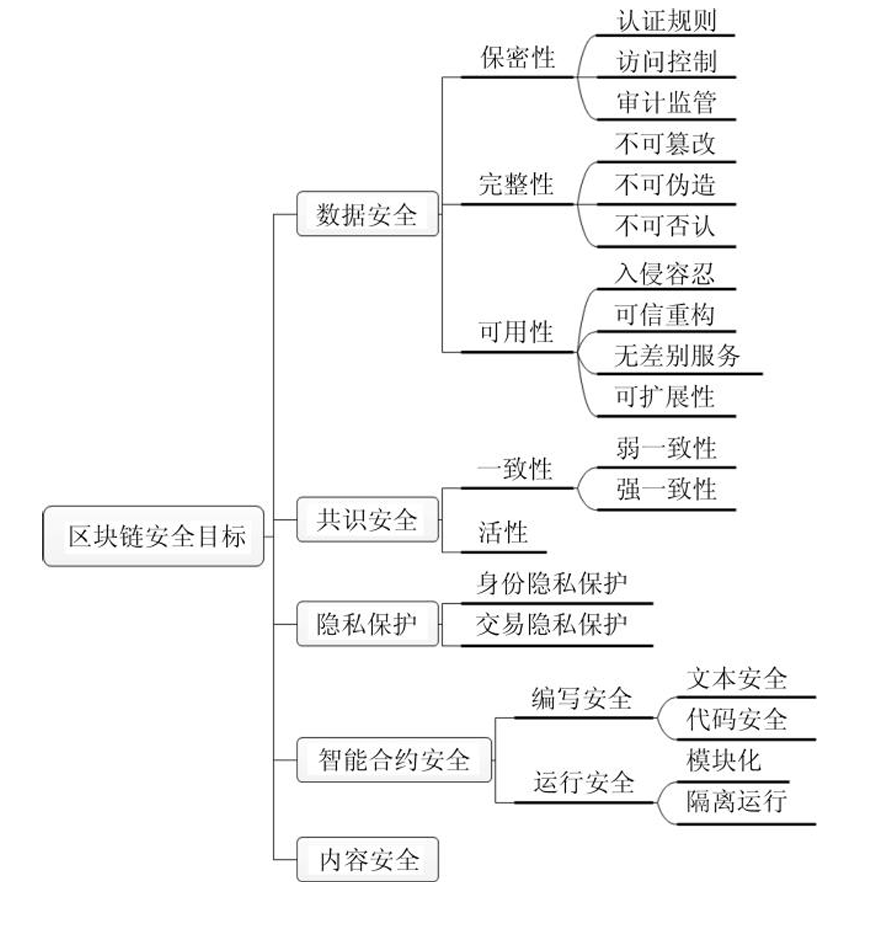
\includegraphics[width=0.5\textwidth]{img/1.png}
	\caption{区块链安全目标}
	\label{fig:example}
\end{figure}

其中, 数据安全是区块链的首要安全目标. 共识安全、智能合约安全、隐私保护和内容安全等安全目标与数据安全联系紧密, 是数据安全目标在区块链各层级中的细化, 也是区块链设计中需要特别考虑的安全要素


section{技术限制与挑战}

为了更好地解释区块链体系结构中提供的安全机制和出现的安全问题, 本文采用《区块链技术发展现状与展望》[6] 中提出的数据层、网络层、共识层、激励层、合约层和应用层六层体系架构, 并以此为基础从信息安全的角度对六层体系架构进行重新解释. 每层可细分为基础模块和安全模块两部分, 如图5.2 所示. 其中, 基础模块是用于实现该层主要功能的基本组件. 安全模块则是用于保障各层安全性, 为上层提供安全稳定技术支持的安全组件。

\begin{figure}
	\centering
	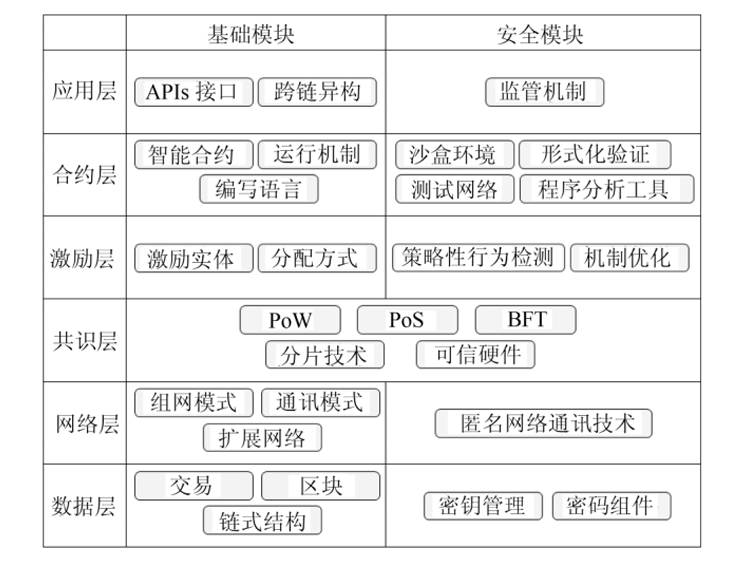
\includegraphics[width=0.5\textwidth]{img/2.png}
	\caption{区块链体系架构}
	\label{fig:example}
\end{figure}

关于区块链的技术限制与挑战,我们使用自底向上方法构建区块链体系架构并阐述每个层级所面临的安全问题。(如同计算机网络的自顶向下方法的七层理论网络) \\


数据层既规定了交易、区块、链式结构在内的狭义区块链的数据结构和存储形式等基本模块, 也包括了关于用户身份、地址的密钥管理机制以及区块链所需的其他密码学组件等安全模块, 是实现其他五层功能的基础. 综合数据层各组件特点, 数据层面临着量子计算威胁、密钥管理不当、交易关联性紧密和密码组件代码漏洞等安全性问题

网络层的核心是确保区块链节点的合法加入和有效通信, 具体包括区块链的组网模式、节点之间的通信模式、扩展网络以及必要的匿名网络通信技术。网络层的安全问题主要包括 P2P 网络的安全问题、网络拓扑被用于攻击以及网络层面的隐私保护问题。

共识层是区块链架构的核心, 主要规定了区块链的共识机制, 确保各节点在网络层提供的网络环境和通信模式中可以共享同一份有效的区块链视图 (View). 区块链的最大创新在于共识层支持的共识机制提供了一种剔除可信第三方的可信数据共享机制, 为上层应用提供安全的账本支持[7]. 

共识层致力于设计高安全性、高效率、低能耗的共识机制, 根据采用的基础协议不同, 可以划分为 5大系列, 包括 PoW、PoS、拜占庭容错协议 (Byzantine fault tolerance, BFT)、分片技术、可信硬件。区块链上的共识机制发展尚不完善, 普遍存在安全性证明不完备、安全性假设不可靠、扩展性差、一致性不稳定、初始化和重构难等问题. 不同类型的共识机制还面临不同的攻击威胁。

激励层需要解决的主要问题是经济学上的激励不相容问题, 具体指参与维护区块链的矿工不会实施危害安全性的恶意攻击, 但是会以自身利益最大化来指导自己的挖矿策略. 这种策略与区块链整体利益形成冲突, 破坏区块链系统效率和稳定性, 包括自私挖矿攻击[8]、Nothing at stake 攻击、扣块攻击 (Withholding attack)[9] 和激励不可持续问题。

合约层由于智能合约代码开源、涉及数字资产转移, 一旦代码漏洞被利用, 会造成不可逆转的损失. 除智能合约创建者在设计业务逻辑时的文本安全问题以外, 合约层还面临智能合约代码漏洞、外部数据源调用、缺乏形式化验证、难实现隐私保护等问题。

区块链在金融、供应链、能源等多领域具有广泛的应用场景(将会在第6节详细叙述). 虽然在不同的应用场景下, 应用层需要反映不同的区块链的业务功能, 在设计上略显差异. 但是, 应用层作为直接与用户交互的区块链层级, 在架构设计上还具有一定的共同点. 一般地, 应用层需要具备 API 接口、跨链异构和监管技术. 从当前区块链应用发展来看, 应用层设计面临跨链操作难、监管技术缺失和应用层攻击等问题.

\begin{figure}
	\centering
	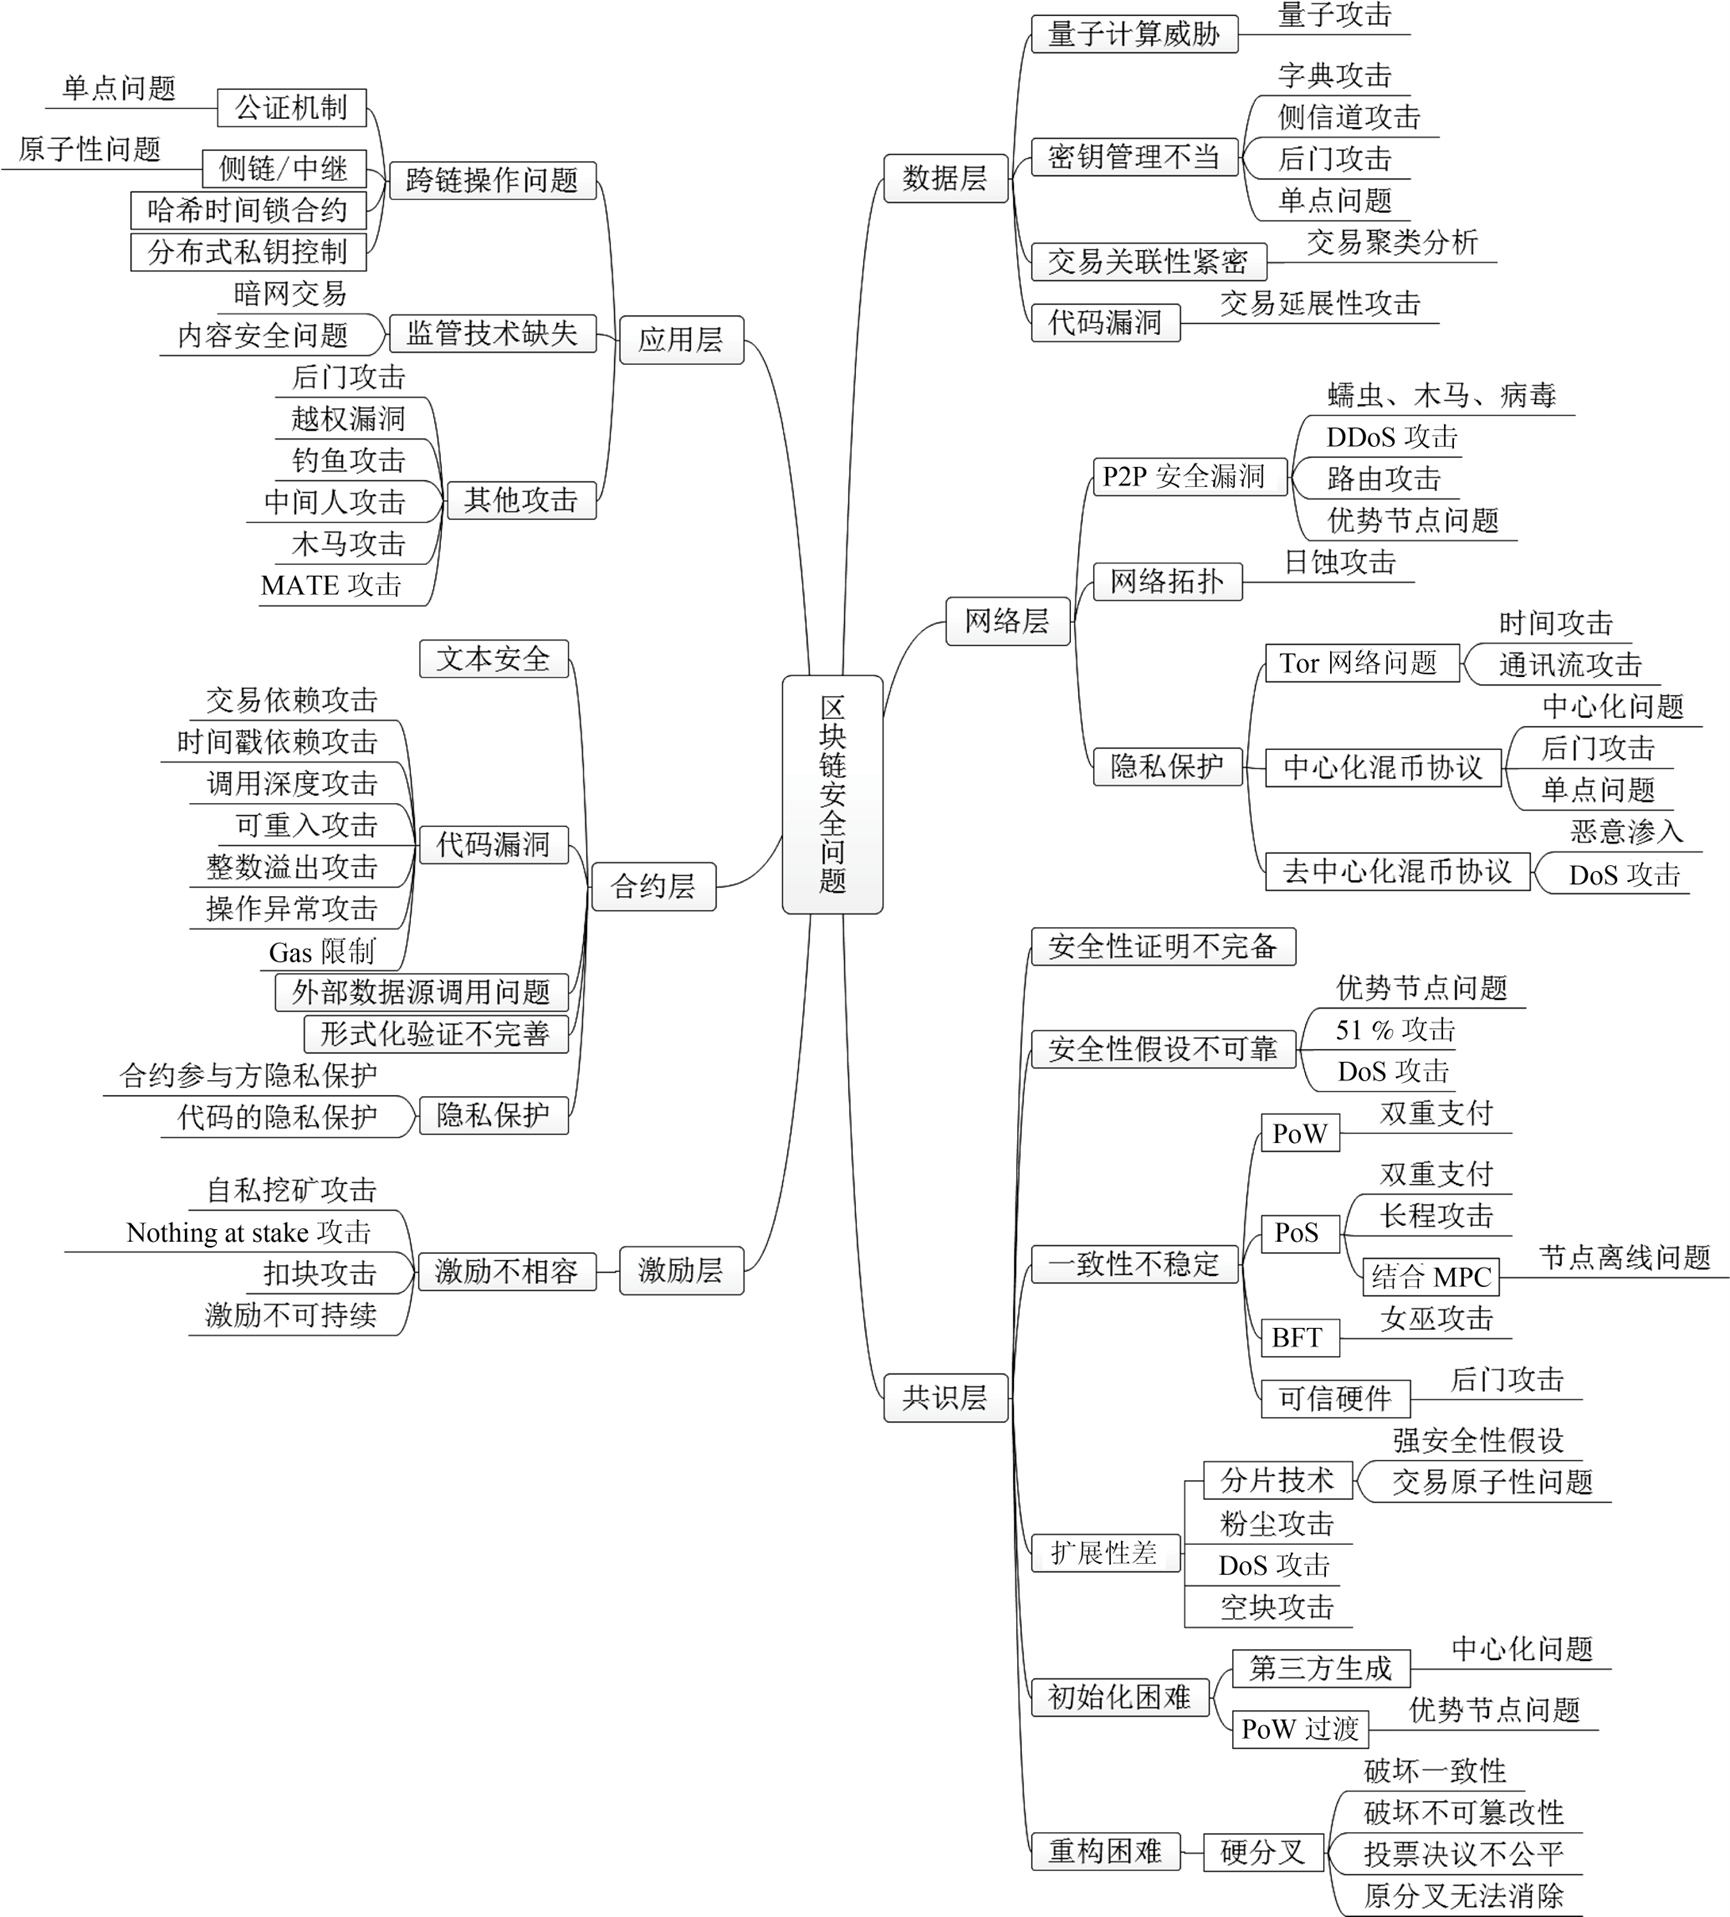
\includegraphics[width=0.5\textwidth]{img/3.png}
	\caption{区块链的安全问题}
	 Fig.3	Security threats on blockchain [10]
	\label{fig:example}
\end{figure}

\section{监管和合规性难题}

由于本小节部分涉及敏感的当地的区块链政策与法律法规,因此使用奥卡姆剃刀原则,抛却本国区块链合规以及跨国区块链监管等跨国政府需要解决的难题,本小节聚焦于作为一个区块链发行商与加密货币拥有者需要解决的监管和合规性难题。 \\

区块链网络作为去中心化的分布式系统, 其各节点在交互过程中不可避免地会存在相互竞争与合作的博弈关系, 这在比特币挖矿过程中尤为明显. 通常来说, 比特币矿池间可以通过相互合作保持各自稳定的收益. 然而, 矿池可以通过称为区块截留攻击 (Block withholding attacks) 的方式、通过伪装为对手矿池的矿工、享受对手矿池的收益但不实际 贡献完整工作量证明来攻击其他矿池, 从而降低对手矿池的收益. 如果矿池相互攻击, 则双方获得的收益均少于不攻击对方的收益. 当矿池收益函数满足特定条件时, 这种攻击和竞争将会造成 “囚徒困境”。 

如何设计合理的惩罚函数来抑制非理性竞争、使得合作成为重复性矿池博弈的稳定均衡 解, 尚需进一步深入研究. 此外, 正如前文提到的, 区块链共识过程本质上是众包过程, 如何设计激励相容的共识机制, 使得去中心化系统中的自利节点能够自发地实施区块数据的验证和记账工作, 并提高 系统内非理性行为的成本以抑制安全性攻击和威胁, 是区块链有待解决的重要科学问题


\section{市场认知与接受度问题}

在中心化社会系统中, 数据通常掌握在政府和大型企业等 “少数人” 手中, 为少数人 “说话”, 其公正性、权威性甚至安全性可能都无法保证.区块链数据则通过高度冗余的分布式节点存储, 掌握在 “所有人” 手中, 能够做到真正的 “数据民主”.就信用基础而言, 中心化社会系统因其高度工程复杂性和社会复杂性而不可避免地会存在 “默顿系统”的特性, 即不确定性、多样性和复杂性, 社会系统中的中心机构和规则制定者可能会因个体利益而出现失信行为;

区块链是实现 CPSS [社会物理信息系统 (Cyber-physical-social systems, CPSS)]平行社会的基础架构之一,其主要贡献是为分布式社会系统和分布式人工智能研究提供了一套行之有效的去中心化的数据结构、交互机制和计算模式, 并为实现平行社会奠定了坚实的数据基础和信用基础。 \\

区块链其核心优势——去除中介和提升透明度——可能对一些传统机构的利益构成威胁。银行、保险公司等中介型机构可能会因为区块链技术的普及而失去市场份额,这导致了这些机构可能对区块链技术的推广持保守甚至抵制的态度。这种市场力量的不平衡,加剧了区块链技术在实践中的推广难度。

除此以外,在民主社会,如何处理和保障对CPSS平行社会抱有敌意的人群(这是的确存在的)的接受度和人权也是一个巨大的问题,毕竟我们不应该使用强制手段去达到一个社会目的,即使它是好的。


\chapter{区块链的应用实践}

\section{金融领域的应用}

金融交易: 区块链技术与金融市场应用有非常高的契合度. 区块链可以在去中心化系统中自发地产生信用, 能够建立无中心机构信用背书的金融市场, 从而在很大程度上实现了 “金融脱媒”, 这对第三方支付、资金托管等存在中介机构的商业模式来说是颠覆性的变革; 在互联网金融领域, 区块链特别适合或者已经应用于股权众筹、P2P 网络借贷和互联网保险等商业模式; 

证券和银行业务也是区块链的重要应用领域, 传统证券交易需要经过中央结算机构、银行、证券公司和交易所等中心机构的多重协调, 而利用区块链自动化智能合约和可编程的特点, 能够极大地降低成本和提高效率, 避免繁琐的中心化清算交割过程, 实现方便快捷的金融产品交易; 同时, 区块链和比特币的即时到帐的特点可使得银行实现比 SWIFT 代码体系更为快捷、经济和安全的跨境转账; 这也是目前 R3CEV 和纳斯达克等各大银行、证券商和金融机构相继投入区块链技术研发的重要原因。


\section{选举投票的应用}

选举投票: 投票是区块链技术在政治事务中的代表性应用. 基于区块链的分布式共识验证、不可篡改等特点, 可以低成本高效地实现政治选举、企业股东投票等应用; 同时, 区块链也支持用户个体对特定议题的投票. 例如, 通过记录用户对特定事件是否发生的投票, 可以将区块链应用于博彩和预测市场等场景[11]; 通过记录用户对特定产品的投票评分与建议, 可以实现大规模用户众包设计产品的 “社会制造” 模式等。


\section{数据鉴证的应用}

数据鉴证: 区块链数据带有时间戳、由共识节点共同验证和记录、不可篡改和伪造,应用于各类数据公证和审计场景. 例如, 区块链可以永久地安全存储由政府机构核发的各类许可证、登记、证明、认证和记录等, 并可在任意时间方便地证明某项数据的存在性和一定程度上的真实性. 包括德勤在内的多家审计公司已经部署区块链技术来帮助其审计师实现低成本和高效地实时审计; Factom公司则基于区块链设计了一套准确的、可核查的和不可更改的审计公证流程与方法[12].


\chapter{区块链的技术发展历程}

\section{区块链的起源与早期发展}

2008年,化名中本聪(Satoshi Nakamoto)发布了比特币的白皮书《比特币:一种点对点的电子现金系统》,提出了一种无需依赖中央银行或中介机构的去中心化数字货币。比特币的核心技术创新就是区块链(如图7.1所示),通过去中心化的分布式账本技术,确保了比特币网络中的交易能够公开透明且无法篡改。

\begin{figure}
	\centering
	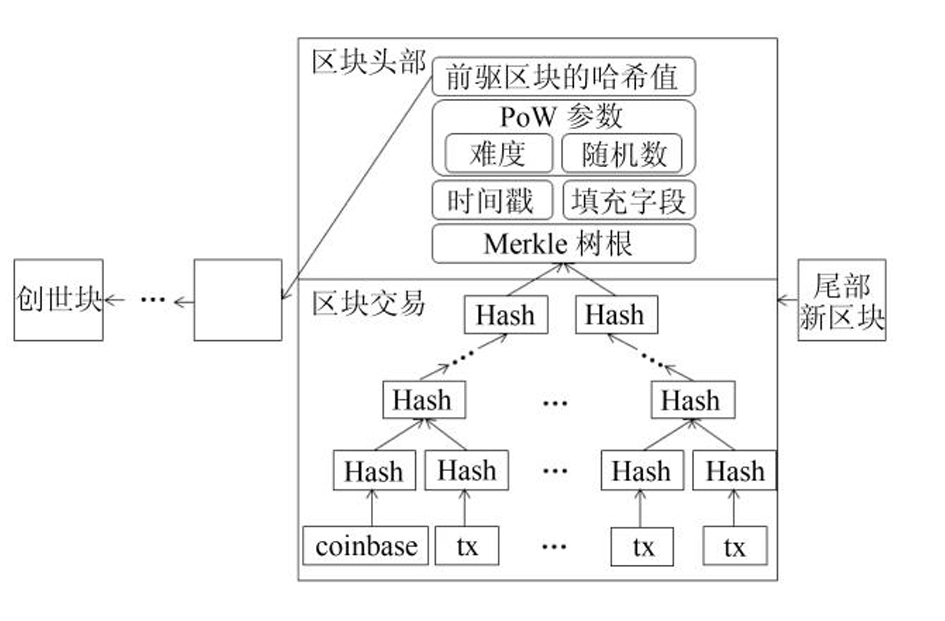
\includegraphics[width=0.5\textwidth]{img/4.png}
	\caption{比特币区块链结构}
	\label{fig:example}
\end{figure}

2009年1月,比特币的创世区块(Genesis Block)被成功挖出,标志着区块链技术的正式诞生。比特币区块链利用“工作量证明”(Proof of Work,PoW)机制保障数据的安全性和不可篡改性。

\section{关键技术突破与演进}

自从早期区块链交易之后,区块链的关键技术突破主要包括共识机制的创新(如从PoW到PoS)、智能合约的应用与优化、侧链与跨链技术的进展、隐私保护技术(如零知识证明)的发展,以及可扩展性和性能的提升(如分片技术)等。

以下从两个我感兴趣的方面入手(毫无疑问,我无法写出所有的技术突破)介绍关键技术突破与演进,即共识机制的创新(如从PoW到PoS),和零知识证明(在深圳大学区块链宣讲上提问但没有得到满意解答)。

\subsection{共识机制的创新(如从PoW到PoS)}

在PoW机制下,矿工通过计算复杂的数学难题来获得新区块的打包权(即生产新区块)。解决这些难题需要大量的计算能力和能源,矿工需要不断地进行哈希计算,直到找到一个符合要求的哈希值(称为“挖矿”)。

PoS机制通过将区块生产的权力分配给持有大量代币的用户,而不是通过算力竞赛来竞争新区块。具体来说,节点根据其持有的代币数量(或称为“股权”)来决定是否能够打包新区块。持有更多代币的人更有可能被选中创建新区块。

\subsection{隐私保护技术(如零知识证明)的发展}

零知识证明最早由\textbf{Shafi Goldwasser}、\textbf{Silvio Micali}和\textbf{Charles Rackoff}在1980年代提出。其基本思想是:证明者能够向验证者证明某个陈述是正确的,而不需要透露任何与陈述本身相关的具体信息。通过这一机制,能够保护交易、身份等敏感信息的隐私。 \\

\textbf{零知识证明的早期发展历程}

早期的ZKP(交互式零知识证明):最初的零知识证明是交互式的,证明者和验证者需要进行多轮互动才能达成验证。虽然这种方法理论上可行,但由于互动过程较为繁琐,因此难以应用到实际的区块链系统中。

非交互式零知识证明(NIZK):为了提高效率,研究人员提出了非交互式零知识证明(NIZK),其中证明者只需生成一个证明,验证者通过对该证明的验证即可确认其有效性。这种方式显著提高了零知识证明的实际应用性,并成为区块链系统中较为常见的形式。

\textbf{零知识证明的技术突破} \\
(这里仅列出零知识证明的突破,具体证明需要数理逻辑方法,这里不予列出):具体证明参见[13]  \\

•  zk-STARKs(Zero-Knowledge Scalable Transparent Arguments of Knowledge):与zk-SNARKs相比,zk-STARKs不仅提升了隐私保护能力,还增强了可扩展性和透明性。zk-STARKs不依赖于可信设置(如SNARKs中的“可信设置”),这意味着其安全性得到了进一步增强。zk-STARKs能够处理更大规模的数据集,并且适用于更加复杂的计算和证明,因此它在未来的区块链系统中有着广泛的应用前景。

•  Bulletproofs:Bulletproofs是另一种零知识证明协议,旨在提高证明的效率,尤其是针对大规模数据集的场景。Bulletproofs比zk-SNARKs更加灵活,尤其在不依赖于特殊的设置的情况下,它提供了较低的证明大小和较快的验证速度。Bulletproofs在如Monero等隐私保护加密货币中也有应用。





\chapter{不同国家区块链发展现状与社会环境对其研究的影响}

\textbf{1. 美国}

发展现状:美国是全球区块链技术和加密货币发展的领头羊,尤其在金融、科技和创新领域。美国的硅谷、纽约和其他科技中心是区块链初创公司和企业的集中地,推动了该领域的研发和商业应用。美国证券交易委员会(SEC)对加密货币和区块链相关技术的监管逐渐成熟,但也存在政策的不确定性,尤其在如何规范加密货币市场上。

社会环境影响:美国的自由市场经济、创业文化和强大的投资环境对区块链技术的研究和发展起到了积极的推动作用。然而,严格的金融监管和对消费者保护的重视也为区块链的应用和发展带来了一些挑战。


\textbf{2. 中国}

发展现状:中国曾是全球加密货币市场的重要参与者,但随着政府对加密货币的监管和禁令政策逐渐收紧,区块链的应用方向逐步转向了不涉及加密货币的领域。中国政府积极推动区块链技术在金融、供应链、政务服务等领域的应用,并已出台多项支持区块链创新的政策,如推动央行数字货币(CBDC)的研发。许多国有企业和技术公司(如腾讯、阿里巴巴)也在区块链技术上开展了大量研究和应用实验。

社会环境影响:中国的政策主导性特征非常明显,国家对技术创新的支持和对市场的严格管控形成了鲜明对比。在政府的大力支持下,区块链技术的基础研究和应用落地得以加速,但也因政策的不确定性,技术的跨境应用面临一定的困难。

\textbf{3. 欧洲}

发展现状:欧洲各国在区块链技术的应用上保持着较为均衡的进展。德国、瑞士和爱沙尼亚等国家在区块链技术的商业化应用上表现突出,尤其在数字身份、跨境支付、供应链管理等方面取得了显著进展。瑞士的“加密谷”成为区块链和加密货币的全球中心之一,而爱沙尼亚则在数字政府和电子公民服务方面做出了开创性的尝试。

社会环境影响:欧洲各国的社会环境相对稳定,重视数据隐私保护和法律法规的合规性,这使得区块链的研究多集中在合规和透明性上。欧盟也在推动区块链技术的标准化和跨国合作,以提升区块链在全球范围内的互操作性和可扩展性。

\textbf{4. 日本}

发展现状:日本是全球首个全面接受比特币作为法定支付工具的国家。日本政府对区块链技术持积极态度,推动了区块链在金融、供应链、医疗等多个领域的应用。日本的金融行业,尤其是大型银行,已经开始在区块链技术上进行广泛的试验和实施。

社会环境影响:日本有着成熟的技术基础和高度发达的金融体系,社会对新技术的接受度较高。与此同时,日本的严格法规和对金融安全的重视促使区块链技术在合法合规框架下进行创新。这使得日本成为了区块链技术应用的全球示范。




% 其他部分
%\backmatter

% 参考文献
\bibliography{ref/refs}  % 参考文献使用 BibTeX 编译
% \printbibliography       % 参考文献使用 BibLaTeX 编译

% 附录
% 本科生需要将附录放到声明之后,个人简历之前
\appendix
% \input{data/appendix-survey}       % 本科生:外文资料的调研阅读报告
% \input{data/appendix-translation}  % 本科生:外文资料的书面翻译
%\input{data/appendix}

% 致谢
%\input{data/acknowledgements}

% 声明
% 本科生开题报告不需要
%\statement
% 将签字扫描后的声明文件 scan-statement.pdf 替换原始页面
% \statement[file=scan-statement.pdf]
% 本科生编译生成的声明页默认不加页脚,插入扫描版时再补上;
% 研究生编译生成时有页眉页脚,插入扫描版时不再重复。
% 也可以手动控制是否加页眉页脚
% \statement[page-style=empty]
% \statement[file=scan-statement.pdf, page-style=plain]

% 个人简历、在学期间完成的相关学术成果
% 本科生可以附个人简历,也可以不附个人简历
%\input{data/resume}

% 指导教师/指导小组评语
% 本科生不需要
%\input{data/comments}

% 答辩委员会决议书
% 本科生不需要
%\input{data/resolution}

% 本科生的综合论文训练记录表(扫描版)
% \record{file=scan-record.pdf}

\end{document}
